\section{Assignment 2: Basic Probabilities and Visualizations}

\subsection{$\xi$ values}

\begin{itemize}
    \item $\xi_4 = 1$
    \item $\xi_5 = \frac{2}{3}$
    \item $\xi_6 = 8$
    \item $\xi_7 = \frac{1}{3}$
    \item $\xi_8 = 3$
\end{itemize}

\subsection{Problem statement}
\subsubsection*{apparition time of an owl}
Let $Y$ be the random variable with the time it takes to hear an owl (in hours).
The probability density function of $Y$ is given by:
\begin{equation}
    Y(t)=\xi_{5} \exp{-\xi_{6} \sqrt{t]} + \xi_{7} \exp{-\xi_{8} \sqrt[3]{t}}
\end{equation}

\subsubsection*{event probability}

From $Y(t)$, we can derive the probability of the event 'hearing an owl', and more precisely its probability density function $P(t)$::

\begin{equation}
    pdf_{event}(t) = \dv{t} (1-P(t))
\end{equation}

\subsection{probability to wait 2-4 hours to see the event}

this probability is given by substracting $Y(4)$ from $Y(2)$. The result is $0.0048$.
\begin{figure}[h]
\centering
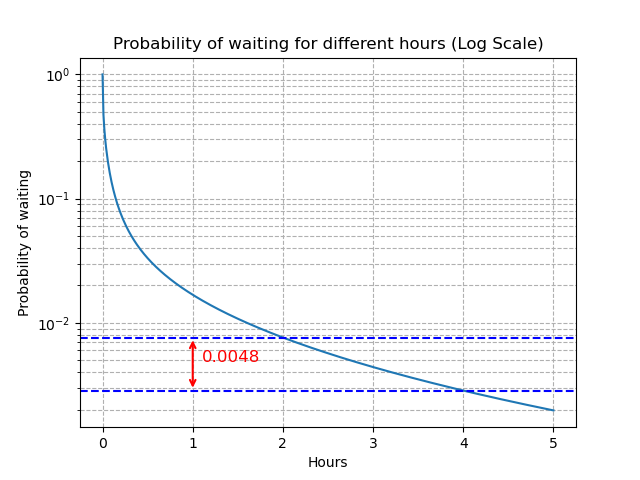
\includegraphics[width=8cm]{code/figures/waiting_time.png.png}
\caption{the probability to wait between 2 and 4 hours is $0.0048$ \label{fig:waiting}
\end{figure}
\FloatBarrier

\subsubsection{event probability density graph}

The graph of the probability density function of the event is given in figure~\ref{fig:waiting}.
\begin{figure}[h]
\centering
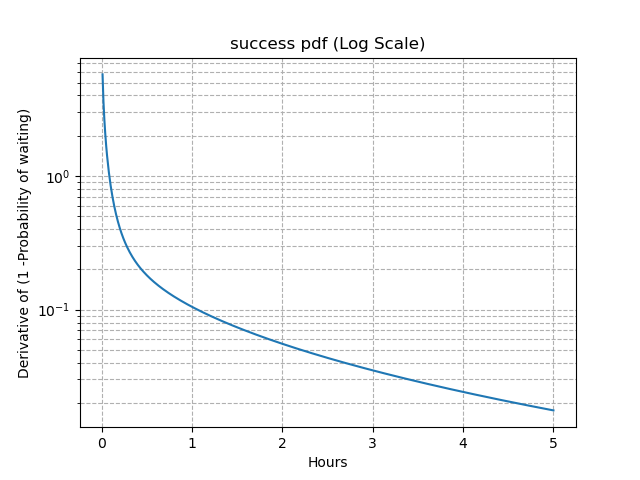
\includegraphics[width=8cm]{code/figures/waiting_time_derivative.png.png}
\caption{the probability density function of the event \label{fig:waiting}
\end{figure}
\FloatBarrier
